\section{Task: Manage Data Sources}
\label{sec:task_manage_datasources}

This task allows management of data sources, as stored in the configuration as well as the database. It can not be run, but is performed using the GUI elements. \\

It is recommended if (in database data sources) position information is missing for a Radar, or a data source name is the same as the id number (default name for unknown data sources).

\begin{figure}[H]
  \hspace*{-2.5cm}
    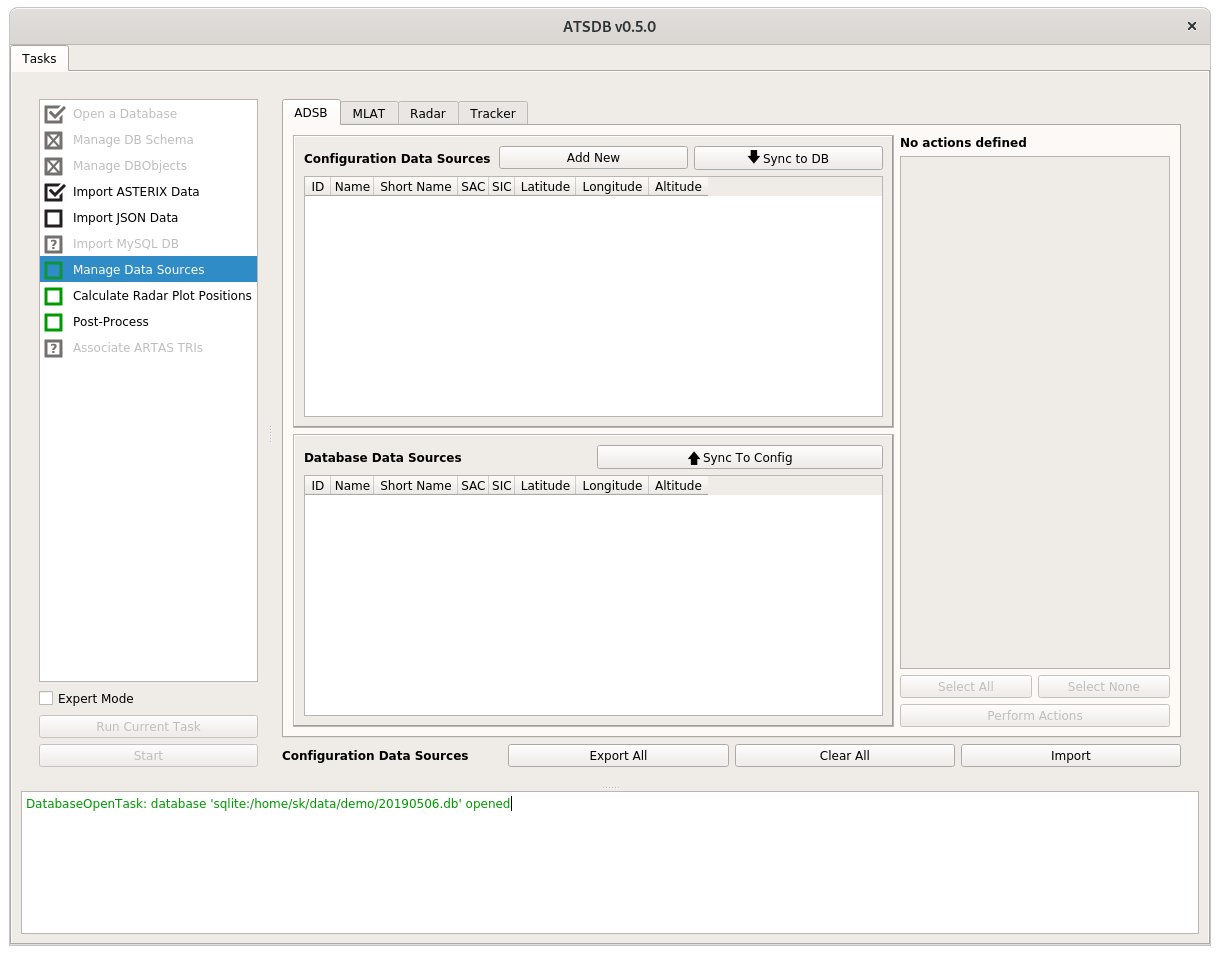
\includegraphics[width=19cm]{../screenshots/manage_data_sources.png}
  \caption{Task: Manage Data Sources}
\end{figure}

If a SASS-C database is opened, the data sources will be already defined. But if data is imported from ASTERIX or JSON, data source information might be missing, so this information must either be edited manually, loaded from a previous SASS-C evaluation or a previous configuration. \\

A configuration data source is stored in the configuration, which means it is persisted and can be used in all databases. It is useful to define all existing data sources in the configuration, since they are immediately used during import of data. \\

A database data source is stored in the database only. During the import, if a data source can be found (matching SAC/SIC) in the configuration, it is automatically added as a database data source. \\

Please \textbf{note} that currently the position of data sources is only required for \textbf{Radar} data sources (in the plot position calculation), for the others it would suffice to have SAC/SIC and name information for display purposes.

At the top, tabs are created for each DBObject, which allow management of the respective data sources. On the bottom, buttons exist to allow functions to work on \textit{all} configuration data sources.

\paragraph {DBObject Tabs}

At the top, the data sources in the configuration are shown and can be managed. 

On the right hand side, available synchronization actions are shown. They can be created, checked, edited or disabled before executing. \\

At the bottom, the data sources as existing in the currently opened database are shown and can also be edited, as well as synchronized to the configuration. \\


\subsection{Editing Database Data Sources}

If ASTERIX/JSON data was imported without stored data source information in the configuration, this would look as follows:

\begin{figure}[H]
  \center
    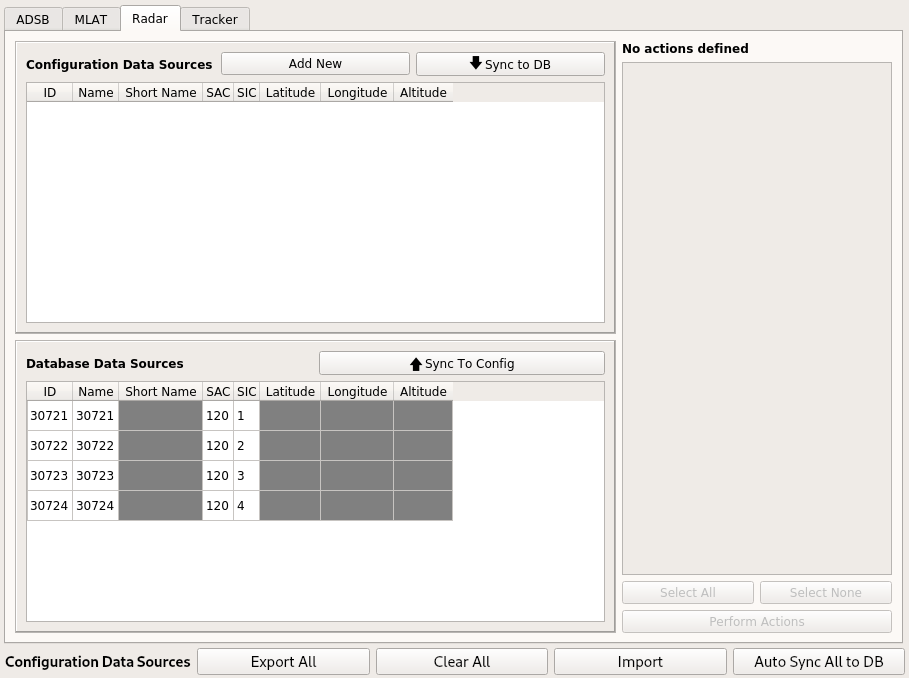
\includegraphics[width=16cm,frame]{../screenshots/manage_data_sources_edit_ds_db.png}
  \caption{DBObject edit data sources in database}
\end{figure}

The gray fields represent the NULL value, to indicate that this information is not (yet) given. Each of the fields can edited, except for the ID field. \\

In a SASS-C database, all of the values would be set. The same can be achieved by editing. Simply click on the value which should be changed, enter a correct value and press return. \\

\begin{figure}[H]
  \center
    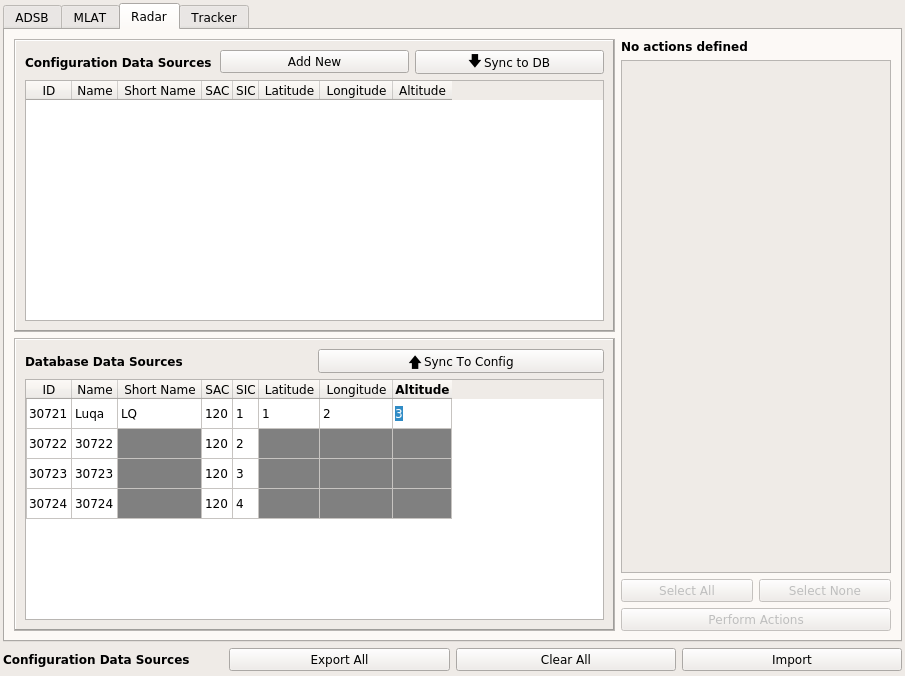
\includegraphics[width=16cm,frame]{../screenshots/manage_data_sources_edit_ds_db2.png}
  \caption{DBObject data sources in database editing}
\end{figure}

All changes made to database data sources are persisted immediately, or reset to NULL if the entered value can not be used (wrong format).

\subsection{Synchchronizing Database Data Sources to Config}

Now, with the already defined data sources, the values should be persisted in the configuration. To achieve this, click on the 'Sync to Config' button to create the proposed actions.

\begin{figure}[H]
  \center
    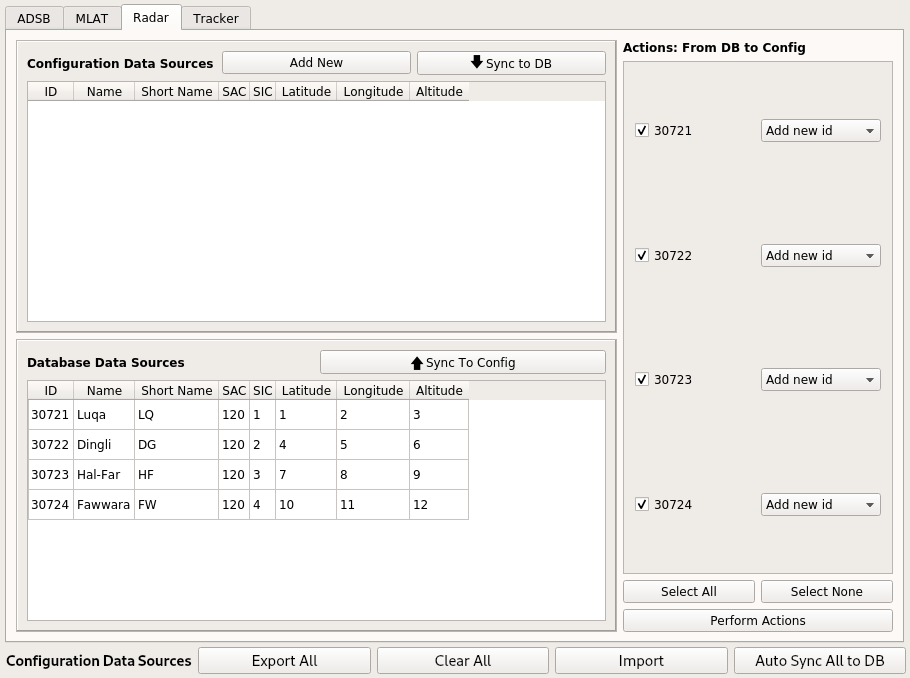
\includegraphics[width=16cm,frame]{../screenshots//manage_data_sources_edit_ds_sync2cfg.png}
  \caption{DBObject synchronize DB data sources to configuration }
\end{figure}

Since no previous data sources are exist in the configuration, the proposed action is to add all data sources as new ones. Unwanted actions can be disabled with the checkbox or set to 'None' in the drop-down menu. To perform the selected action, click the 'Perform Actions' button.

\begin{figure}[H]
  \center
    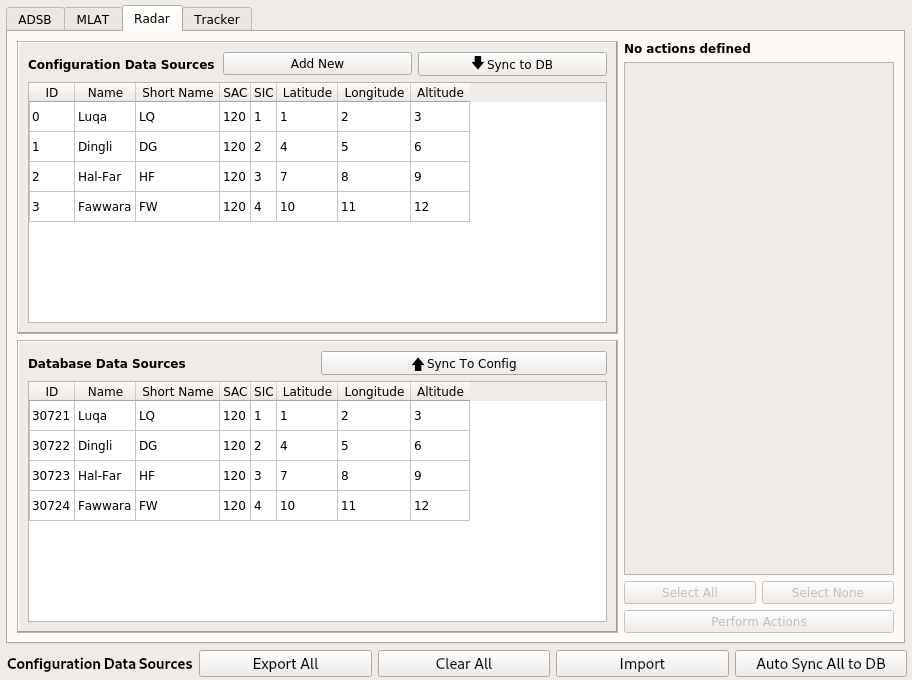
\includegraphics[width=16cm,frame]{../screenshots/manage_data_sources_edit_ds_db2cfgsynced.png}
  \caption{DBObject DB data sources synchronized to configuration }
\end{figure}

\subsection{Editing Configuration Data Sources}

The configuration data sources displayed at the top can also be edited, to change names or correct information. \\

A new one can be added using the 'Add New' button, and then edited by clicking on the respective field. \\

\begin{figure}[H]
  \center
    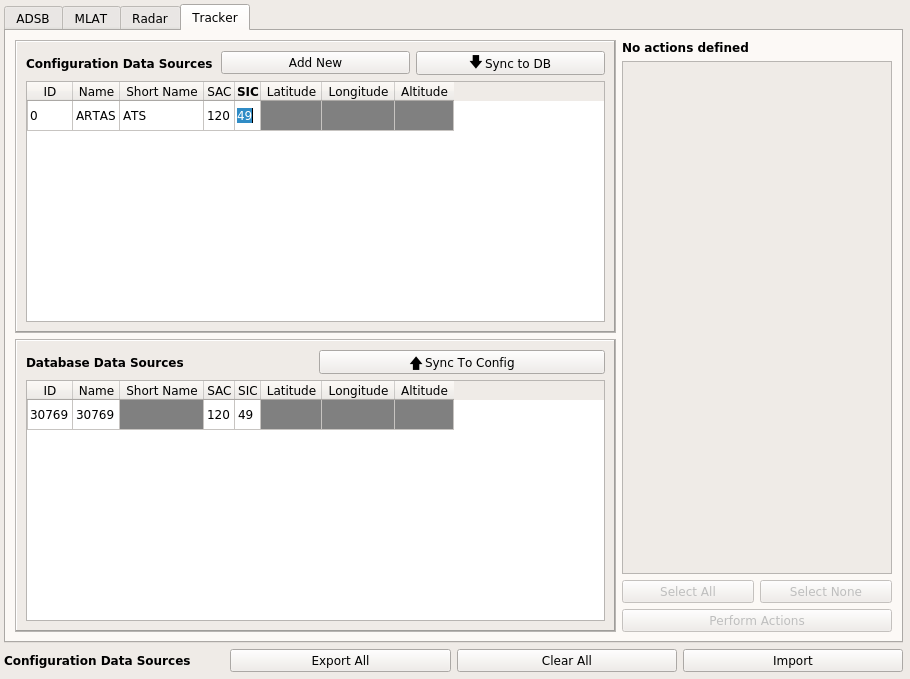
\includegraphics[width=16cm,frame]{../screenshots/manage_data_sources_edit_ds_cfg.png}
  \caption{DBO Edit Data Sources in Configuration}
\end{figure}

If values are changed, the changes will be persisted on correct shutdown of the application.

\subsection{Synchchronizing Configuration Data Sources to DB}

In the previous step values were changed. To synchronize these changes to the currently opened database, click on the 'Sync to DB' button.

\begin{figure}[H]
  \center
    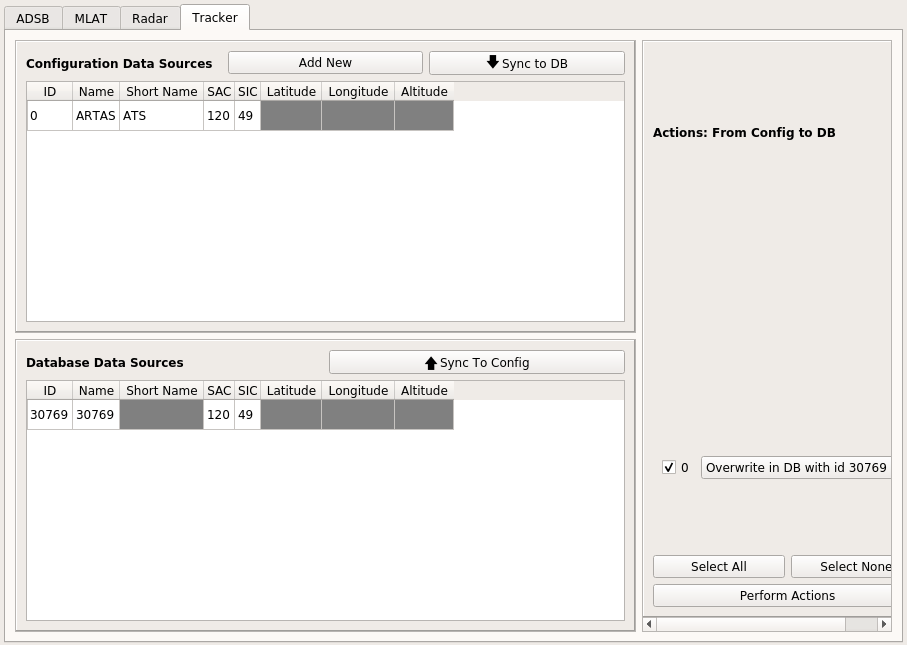
\includegraphics[width=16cm,frame]{../screenshots/manage_data_sources_edit_ds_sync2db.png}
  \caption{DBObject synchronize configuration data sources to DB}
\end{figure}

Note that the proposed action is to overwrite the data source information, since a matching SAC/SIC was found. To perform the selected actions, press the 'Perform Actions' button.

\begin{figure}[H]
  \center
    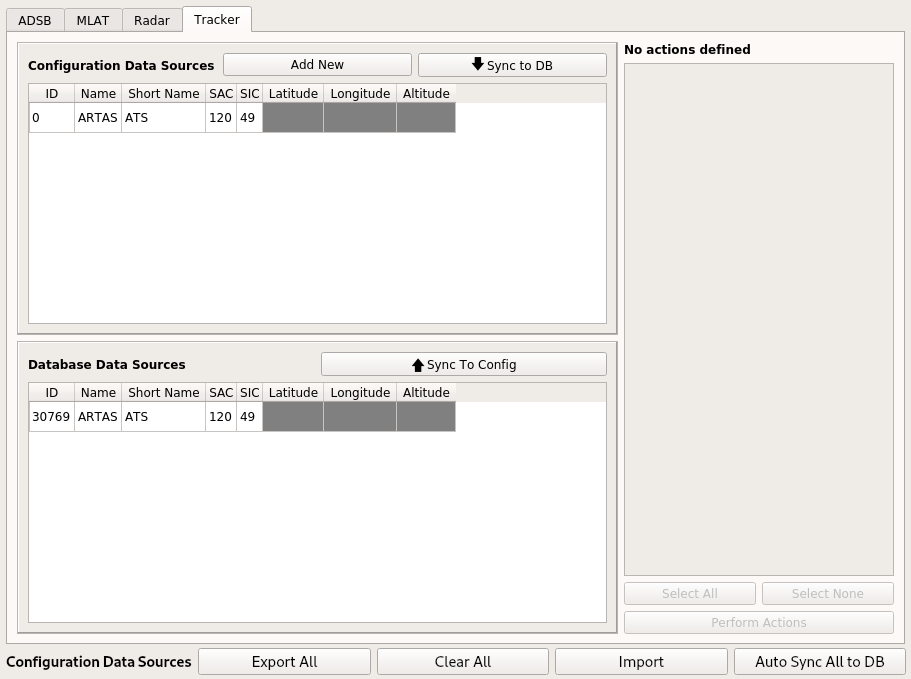
\includegraphics[width=16cm,frame]{../screenshots/manage_data_sources_edit_ds_cfg2dbsynced.png}
  \caption{DBObject configuration data sources synchronized to DB}
\end{figure}

Please \textbf{note} that, if all database data sources are set correctly (Radars have positions and all data sources have names not being their id value), the task is assumed to be performed and the next recommended task is selected. However, if further editing is wanted, this task can be re-visited using the task list.

\subsection{Import/Export of Configuration Data Sources}
\label{sec:config_ds_export}

Using the 3 buttons on the bottom the following functions can be used:

\begin{itemize}  
\item Export All: Export all configuration data sources from all DBObjects as JSON file
\item Clear All: Delete all configuration data sources from all DBObjects
\item Import: Import configuration data sources for all DBObjects from JSON file
\end{itemize}
\ \\

An exported JSON file can look as follows:

\begin{cverbatim}
{
    "Radar": [
        {
            "altitude": 3.0,
            "dbo_name": "Radar",
            "latitude": 1.0,
            "longitude": 2.0,
            "name": "Luqa",
            "sac": 120,
            "short_name": "LQ",
            "sic": 1
        },
        {
            "altitude": 6.0,
            "dbo_name": "Radar",
            "latitude": 4.0,
            "longitude": 5.0,
            "name": "Dingli",
            "sac": 120,
            "short_name": "DG",
            "sic": 2
        },
        {
            "altitude": 9.0,
            "dbo_name": "Radar",
            "latitude": 7.0,
            "longitude": 8.0,
            "name": "Hal-Far",
            "sac": 120,
            "short_name": "HF",
            "sic": 3
        }
    ],
    "Tracker": [
        {
            "dbo_name": "Tracker",
            "name": "ARTAS",
            "sac": 120,
            "short_name": "ATS",
            "sic": 49
        }
    ]
}
\end{cverbatim}

Using these functions, the configuration data sources can be changed for sensor context switches, or e.g. exported before an ATSDB version upgrade.

\subsection{Comments}

This procedure  has to be performed once for each DBO, after that the data sources are defined in the configuration. Also, if you have access to a SASS-C database, it is easier to synchronize the data source information from there to the configuration. \\

After doing so, for imported JSON/ASTERIX the SAC/SIC information supplied in the target reports is used to match them to the respective data source. \\

For matching purposes only the SAC/SIC values are of importance, the name information doesn't have to be unique. If multiple data sources identical SAC/SIC values exist (for whatever reason), the first match is used during import. 
